
% This chapter presents the implementation of a distributed system running on Matrix and developed with Paragon as described in the criterias.

This chapter describes the implementation of the prototype in the case study. The prototype is a system for sending and retrieving patient journals among different hospitals. The system relies on Matrix as the secure communication channel and storage.


\section{Journal system}

% Describe the requirements for the journal system.
A journal system serves an important purpose by providing patient journals to different hospitals and clinics. If a patient arrives at the ER and the doctor cannot access the patient's journal then the treatment of the patient gets problematic. A doctor might miss out on important details about the patient or even worse prescribe medication that might give the patient an allergic reaction. The availability of a patient journal is a necessity however the number of medical employees that have access to such a journal has raised privacy concerns. Around 90.000 medical employees have access to patient journals. Consider the scenario where a patient gets referred to a physiotherapist with muscle pain. When the therapist opens the journal the full medical history will be present; if the patient had received psychiatric treatment those session would be readable too. Furthermore a patient journal is accessible by a large number of unrelated medical employees with the only prevention mechanism being logging and audit trails.


The lack of secure information flow is evident and the prototype demonstrates how Information-Flow control can be leveraged to enforce security policies concerning the information. The journal system is a small distributed system where Hospitals can send, receive and store patient journals. Matrix provides the distributed structure and is responsible for securely storing and transmitting the journals. Paragon provides secure information flow at the endpoints hence providing end-to-end security. 
The following requirements are defined for the prototype:

\begin{itemize}
	\item A patient journal contains low (public), medium (confidential) and high (secret)  information.
	\item A patient journal is send and received securely over a channel.
	%\item A patient journal can only be appended to. 
	\item Hospitals have shared access to patient journals. 
	\item A hospital has two actors: Doctor and Secretary.
	\item A secretary can only see low parts of the journal.
	\item A secretary can edit the public parts of a journal.
	\item A doctor can see the everything up to confidential information.
	\item A doctor must have the patient in care to gain the journal's secret information.
	\item A doctor can edit the public part and confidential parts of a patient journal.
	\item A doctor can only add to a secret fields in a patient journal if the patient has been referred to the doctor.
\end{itemize}

The following non-functional requirements are defined:

\begin{itemize}
	\item Confidentiality: the system must ensure the confidentiality throughout the system according to the security policies at all times.
	\item Integrity: the system must ensure that only intended actors can modify the specific parts of a patient journal.
	\item Accessibility: the system can only used from the hospital hence retrieving patient journals outside the hospital is not possible.
\end{itemize}


\subsection{System design} \label{systemdesign}


The system consists of two components; \emph{Matrix} and the \emph{client}. The Matrix component encapsulates the Matrix SDK and provides an interface. The client component consumes that interface and can be considered as the endpoint in a communication channel. The client component provides secure information flow for data received through Matrix. 
The component diagram in figure \ref{fig:matrix_component} depicts this.

\begin{figure}[H] 
	\hspace*{-1cm}
	\centering
	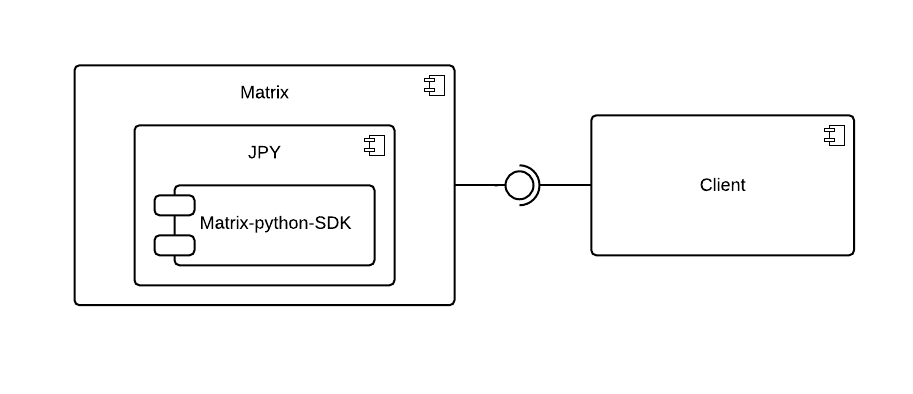
\includegraphics[width=14cm]{figures/matrix_component.png}
	\caption{Component diagram for the system}
	\label{fig:matrix_component}
\end{figure}

Matrix provides several SDK libraries that client application can be build on top of. The most prominent is the Javascript Matrix SDK. It is the best maintained with the largest feature set however it is not compatible with the Java based Information-Flow Control tool Paragon. A Java Matrix SDK exists but it is an early alpha version with end-to-end encryption not implemented yet. The Python Matrix SDK is another major SDK with support for end-to-end encryption in beta. The Python Matrix SDK is used in the Matrix component through a Java-Python bridge \emph{JPY} that can embed Python code in Java as shown in the Matrix component in figure \ref{fig:matrix_component} 


\subsubsection{Matrix}
%Matrix API's
% A lot of things are handled under the hood by the matrix SDK.
Matrix is an important component in the system. It manages the transmission and storage of patient journals through rooms while managing end-to-end encryption. The encryption mechanism is automatically provided and the SDK manages the session keys under the hood.  As described in section \ref{matrix:architecture} a room is a conceptual place for sending an receiving events and events can be any of any structure. The event history in a rooms is replicated at each homeserver. 

The following design choices and assumptions are made regarding Matrix and the system: 

\begin{itemize}
	\item A homeserver represents a hospital server that replicates the history of a patient journal. 
	\item A room represents a single patient journal's version history.
	\item An event represents a patient journal.  
	\item The latest event in a room is the global state of the patient journal.
	\item A hospital is represented by a single matrix user that participates in a room.
	\item A hospital's matrix user is used by doctors and secretaries to access patient journals. 
\end{itemize}


The room can be considerably large since many different types of hospitals needs access to a patient journal. This puts a lot of responsibility on securing the endpoints but also adds concern to who controls the rooms and how hospitals are added. It is assumed that a central authority would be managing all room whom all participants in the room trust. That authority would be the government which are responsible for creating and managing the rooms. Only the authority can invite and remove Hospitals from a room. Hospitals can only join a room if they have been invited.


\subsubsection{Client}

The program starts as either a doctor or a secretary. The user is then presented a list of patients that can be selected. The list is provided by the hospital that keeps track of all journals in a hashmap with \emph{SSN} (Social security number) as the key and \emph{matrix room ID} as the value. When the user selects a journal; it is first retrieved from Matrix and the user then receives the journal. It is determined what tasks the user can perform and depending on the user's role the journal can be partially or fully accessible 

Figure \ref{fig:journalsystem} depicts the class diagram for the system.


\begin{figure}[H] 
	\hspace*{-1.3cm}
	\centering
	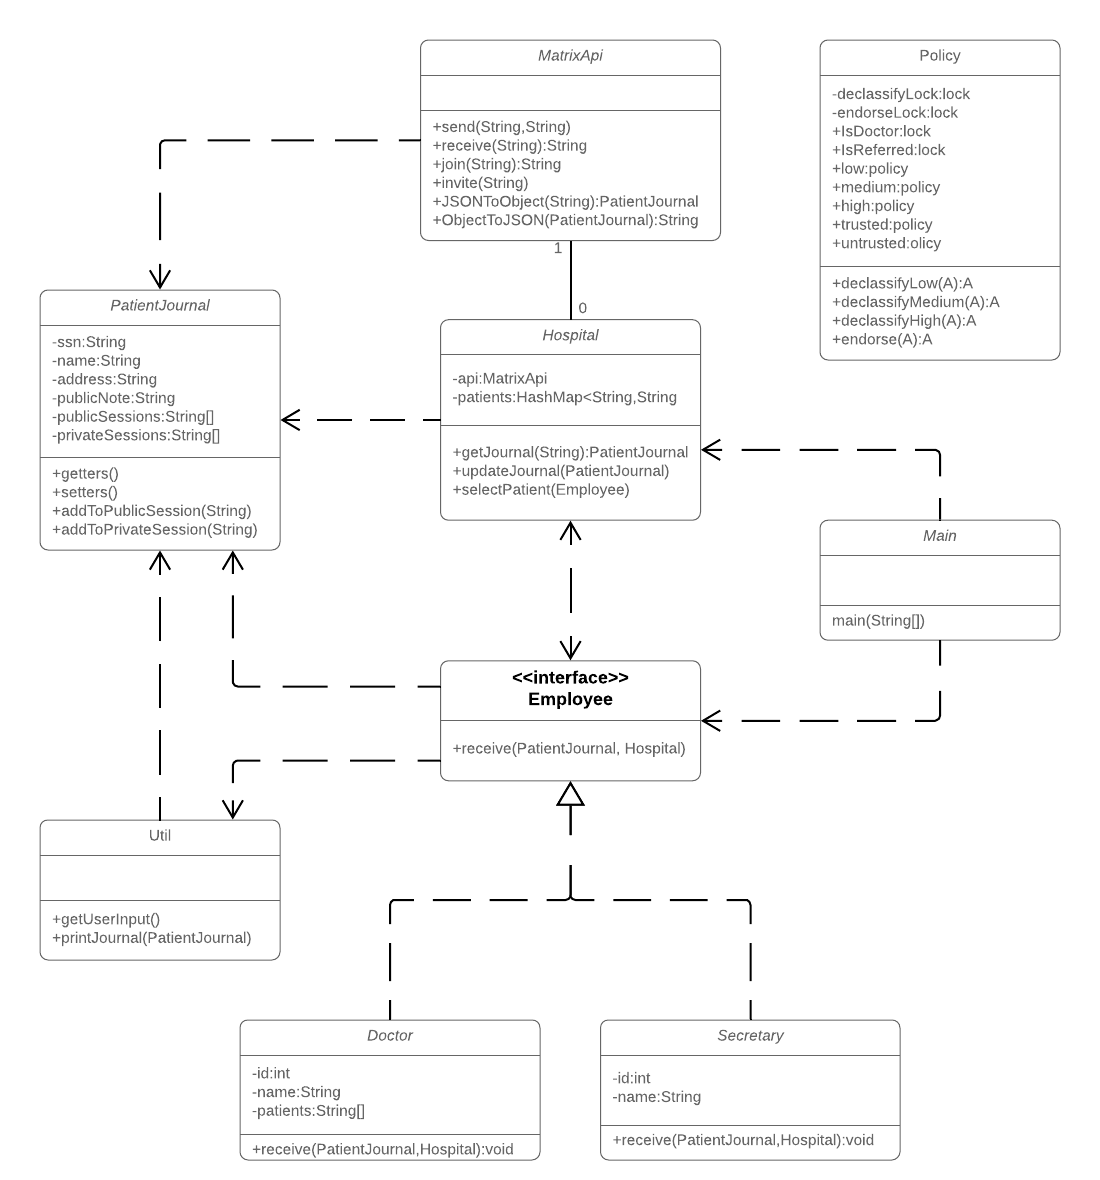
\includegraphics[width=14cm]{figures/journalsystem_class.png}
	\caption{Class diagram for the Journal system}
	\label{fig:journalsystem}
\end{figure}





\subsubsection{Limitations}

%Incompatibility with Paragon


A design problem is the concurrent writes to a journal from multiple hospital. Before writing to a journal; the latest version of the journal in Matrix is first retrieved and then the writes are appended to the journal. However multiple hospitals might have retrieved the latest journal and different doctors might have committed changes to the journal and send it to Matrix hence one of the writes would be lost since only the latest journal is retrieved. 


% It is assumed that a version control mechanism is in place and the latest journal received is always up to date.
% Solution merging data like version control systems like git.

\section{Paragon implementation}

A \emph{policy-first} approach is used when implementing the prototype. The first step is to carefully specify the policies for the system. A journal has several parts that may only be obtained by appropriate users; the policies should uphold that. The policies are defined in the class \emph{Policy} and used throughout the system.

For confidentiality three policies are defined with \emph{low} being the most liberal, \emph{High} being the most strict and \emph{medium} in the middle. The figure \ref{fig:lattice_confidentiality} depicts a lattice for the three policies where information can only flow upwards. In the figure \emph{public} represents low, \emph{confidential} represents medium and \emph{secret} represents high. 

Based on the requirements the information labeled with secret should only be obtainable by the Doctor that the patient has been referred to. There could be defined a similar independent secret labels e.g. for information that only the patient's psychiatrist could view.  

% Show confidentiality lattice and combined lattice.

\begin{figure}[H] 
	\centering
	\includegraphics[width=6cm]{figures/lattice_confidentiality.png}
	\caption{Lattice in the system}
	\label{fig:lattice_confidentiality}
\end{figure}

The lattice in figure \ref{fig:lattice_confidentiality}b illustrates the integrity policy and states that data labeled as \emph{untrusted} can not flow to \emph{trusted}. The trusted and untrusted labels serves the purpose of disallowing flows to the journal.

The fields in the PatientJournal class are decorated with a combination of confidentiality labels. The \emph{product lattice} is illustrated in the figure \ref{fig:lattice_product}.

\begin{figure}[H] 
	\centering
	\includegraphics[width=7cm]{figures/lattice_product.png}
	\caption{Product lattice}
	\label{fig:lattice_product}
\end{figure}


The next section will show how the policies have been defined and used in paragon. 



\subsection{Policies}\label{policies} 

In Paragon a policy defines what actor information can flow to and under what conditions 
\cite{paragonprogramming}. Any object can be used as an actor. The confidentiality policies in the prototype uses \emph{Doctor} and \emph{Secretary} as actors. 


\subsubsection{Defining policies}\label{policydef}
The policies \emph{low}, \emph{medium} and \emph{high} are defined as this:

\begin{lstlisting}
public static final policy low = { Doctor d: ;Secretary s:};
public static final policy medium = { Doctor d:};
public static final policy high = { Doctor d: IsReferred(d)};
\end{lstlisting}


Here policy \emph{low} is less restrictive than \emph{medium} since a variable labeled with the policy low can be viewed by the any\emph{Doctor} or \emph{Secretary} actor whereas a variable labeled with \emph{medium} can only be viewed by any \emph{Doctor} actor. The policy \emph{high} is a more interesting policy. It is more restrictive since it can only flow to a specific \emph{Doctor} if the lock \emph{IsReferred(d)} is open. Policy \emph{high} is an example of a dynamic policy which uses a parameterized unary lock.

The following are integrity policies defined as follows:
\begin{lstlisting}
private static final Object untrustedObserver = new Object();
private static final Object trustedObserver = new Object();
public static final policy untrusted = { untrustedObserver :; };
public static final policy trusted = { untrustedObserver :; trustedObserver: };
\end{lstlisting}


The actors used here are \emph{untrustedObserver} and \emph{trustedObserver}. The policy \emph{trusted} can be viewed by both observers while \emph{untrusted} can only be viewed by \emph{untrustedObserver}. This captures integrity since a variable labeled with \emph{untrusted} can not flow to \emph{trusted}. Note that actors used here are instances of objects and using them as actors gives the policies a special property of being combinable with other policies \cite{paragonprogramming}.


% The policies defined for confidentiality are with fresh actors and the objects correspond to the entities where information may flow. By using fresh actors the policies can be combined with other policies that would otherwise have interfered with eachother. The integrity policy is more general in nature and has defines two actors; trusted and untrusted observers. The policies are defined as follows: ?(Policy.high + Policy.trusted).

% Dynamic policy is used for when a doctor adds notes to session. The lock IsDoctor must be open for the method addToSession() can be invoked. This is checked at runtime as seen in the code snippet:


% Policy definition
% Policy usage
\subsubsection{Using policies}
A policy is used as a label on variables. To express concerns for both confidentiality and integrity the policies described previously can be combined and labeled on variables. Fields in the class \emph{PatientJournal} are defined as:

\begin{lstlisting}
	private ?(Policy.low    + Policy.trusted) String   publicNote;
	private ?(Policy.medium + Policy.trusted) String[] publicSessions;
	private ?(Policy.high   + Policy.trusted) String[] privateSessions;
\end{lstlisting}

The \emph{PatientJournal} class has methods that adds a session to \emph{publicSession} or \emph{privateSession}. The class also implements simple getter and setter methods. Common for these methods are they must specify the \emph{read} or \emph{write} effect for the method.

% Show table of policies and how they are defined and how they are used for low, high and medium.



\subparagraph{Read effects}
The read effect specifies what the information policy is. It has already been introduced when labeling the fields in the \emph{PatientJournal} class. When decorating a method with a read effect signature it simply tells what the policy is for the returned type. Paragon ensures that the policy returned must respect the policies of the field or parameters that are in the context of the method. Through read effects explicit flows are captured across methods and fields. This is an example of how a simple \emph{get()} method is defined in \emph{PatientJournal}.
\begin{lstlisting}
?(Policy.medium + Policy.trusted)
public  String[] getPublicSessions(){
	return publicSessions;
}
\end{lstlisting}

If the read effect instead was \emph{?(Policy.low+Policy.trusted)} then Paragon would have caught it since the field \emph{publicSession} has a more restrictive policy. Note that is a read effect is not specified then Paragon sets the read effect as \emph{?(Object x:)} (the least restrictive policy in Paragon).

\subparagraph{Write effects}
In Paragon the write effect prevents implicit flows. The write effect specifies what context the method can be called in. The context would have to at least as restrictive as the method write effect. The write effect for a method is defined like this:

\begin{lstlisting}
!(Policy.low + Policy.trusted) 
public void setPublicNote(?(Policy.low + Policy.trusted) String note){
	this.publicNote = note;
}
\end{lstlisting}

This method has the write effect \emph{!(Policy.lowD+Policy.trusted)}. Now if this method was called in a method that has the write effect \emph{!(Policy.highD+Policy.trusted)} then there would be an implicit flow and Paragon would detect it.

Read and write effects are important aspect of Paragon since they ensure secure information flow across methods and fields.

\subsection{Locks}
The integrity policy ensures that no information can not flow from untrusted source to variables labeled with \emph{trusted}. However we also want to specify which actors are allowed to change information. A secretary should only be able to edit the field \emph{publicNote} in \emph{PatientJournal}. A doctor should be able to add sessions to \emph{publicSessions} but should only be able to add sessions to \emph{privateSessions} if the patient is referred to the Doctor. This has been achieved through locks. The lock \emph{IsReferred} was introduced when defining the \emph{high} policy. The lock takes a \emph{Doctor} as parameter and becomes open for the doctor. Another parameterized lock is the\emph{IsDoctor} lock that opens during program start if the user is a doctor. The locks are accompanied with 0-ary locks \emph{ReferredLock} and \emph{DoctorLock}. The locks are defined as the following: 

\begin{lstlisting}
public static ?(lowD+trusted) lock IsReferred(Doctor); 
public static ?(lowD+trusted) lock ReferredLock;
public static ?(lowD+trusted) lock IsDoctor(Employee);
public static ?(lowD+trusted) lock DoctorLock;
\end{lstlisting}

The locks \emph{ReferredLock} and \emph{DoctorLock} are used on methods with a special annotation that specifies that the method can only be called if the lock is open. By using lock combined with the annotation the requirement for modifying information can be fulfilled. The class \emph{PatientJournal} provides two methods for adding sessions with the annotation:

\begin{lstlisting}
~Policy.DoctorLock
public !(Policy.mediumD + Policy.trusted) void addToPublicSessions(?(Policy.mediumD + Policy.trusted) String session){
// Add sessions
} 

~Policy.Referred
public !(Policy.highD + Policy.trusted) void addToPrivateSessions(?(Policy.highD + Policy.trusted) String session){
// Add sessions
} 	
\end{lstlisting}  

The lock \emph{DoctorLock} is opened when \emph{IsDoctor} is opened and the lock \emph{ReferredLock} opens when \emph{IsReferred} is open. 

% How a lock is opened 
The Paragon compiler might not be able to infer if the lock is opened through compilation. Hence the lock must be checked at run-time and used like this:

\begin{lstlisting}
if(Policy.IsReferred(self)){
	journal.addToPrivateSession(session);
}
\end{lstlisting}



\subsection{Declassification}
A journal system must be able to view the patient journals through some output channel. Furthermore the system must take user input through an input channel to edit a journal. Hence it is necessary to \emph{declassify} information when using an output channel and \emph{endorse} information when using an input channel. The system provides mechanism for achieving this. We need to revisit the policy definitions to make this possible. 

The policy for \emph{System.out} is the least restrictive defined as \emph{?{Object a:}}.
Hence any flow using the defined policies would be rejected. Declassification of information must be done for allowing flow to \emph{System.out}. To achieve this we have to extend the policies with a lock \emph{declassifyLock}:

\begin{lstlisting}
private lock declassifyLock;
public static final policy low = { Doctor d: ;Secretary s:; Object x: declassifyLock};
public static final policy medium = { Doctor d:; Object x: declassifyLock};
public static final policy high = { Doctor d: IsReferred(d); Object x: declassifyLock};
\end{lstlisting}

After the modification the policy now states that a variable labeled with the policy can flow to any actor if the \emph{declassifyLock} is open. Thus we can specify a method that takes some value as input, opens the lock and returns the value with the least restrictive policy:

\begin{lstlisting}
?bottom
public static <A> 
A declassifyLow(?(bottom*low) A x){
	open declassifyLock {
		return x;
	}
}
\end{lstlisting}

The method expects a parameter with a policy that is at least as restrictive as the policy \emph{low} and \emph{bottom} (variable name for {Object x:}). The method opens the lock and returns the variable and has the read effect \emph{?bottom}.  We provide similar declassify methods for \emph{low} and \emph{high}. However it is an issue that a secretary could call declassify methods for \emph{medium} and \emph{high}. We can use the annotation seen in the previous section to overcome this so only the appropriate actors can declassify:

\begin{lstlisting}
~Referred
?high
public static <A> 
A declassifyHigh(?(high*low) A x){
	open declassifyLock {
		return x;
	}
}
\end{lstlisting}

The approach for endorsement is similar with an \emph{endorseLock} added to the \emph{untrusted policy} and then specifying a method that can endorse a variable.

Declassification and endorsement are methods that should be applied with great care. It should be considered who can declassify, what is declassified, where the declassification occurs and when it can occur. The table below gives an overview of this.

\begin{table}[H]
	\hspace*{-2.3cm}
	\centering
	\begin{tabular}{|l|l|l|l|l|} 
		\hline
		& Who               & What                    & Where                                                                         & When                       \\ 
		\hline
		& Anyone~           & Journal.name            & Util.printJournal()                                                           & Printing the journal       \\
		& Anyone~ ~         & Journal.ssn             & Util.printJournal()                                                           & Printing the journal       \\
		Declassification & Anyone~ ~         & Journal.address         & Util.printJournal()                                                           & Printing the journal       \\
		& Anyone~ ~         & Journal.publicNote      & Util.printJournal()                                                           & Printing the journal       \\
		& Doctor            & Journal.publicSessions  & Util.printJournal()                                                           & Printing the journal       \\
		& Doctor (Referred) & Journal.privateSessions & Util.printJournal()                                                           & Printing the journal       \\ 
		\hline
		Endorsement      & Anyone            & User input              & \begin{tabular}[c]{@{}l@{}}secretary.receive()\\doctor.receive()\end{tabular} & After prompting for input  \\
		\hline
	\end{tabular}
\end{table}



%\subsubsection{Lattice}

\subsection{Limitations}

\subsubsection{Matrix API}
The Matrix API implementation was briefly described in section \ref{systemdesign}. The API is implemented in Java using the foreign language binder JPY to leverage the Matrix Python SDK and makes it possible to use it with Java/Paragon. When a journal is passed to the API the encryption is not performed until the Python code is executed. Hence there exists a layer between Paragon and Matrix where the data is unencrypted and where Paragon policies cannot be enforced.

\subsubsection{Exception handling}
Another limitation of the prototype is that exceptions are unexplored. Any exception is a potential channel for implicit flows. The tools provided by Paragon such as read effects, write effects and locks can be used to properly handle exception.





\section{Summary}
This chapter has described requirements for the prototype, the overall system design and how it is implemented in Paragon. We have seen how the policies can be described and enforced in Paragon. 